% ResumenProyecto.tex
% ========================
%
%
% Descripción:
% ------------
% Documento para enviar al Dr Pomares
%
%
%
%
% Metadatos:
% ----------
% * Autor: zxxz6 (Bryan Violante Arriaga)
% * Versión: 1.0.0
%
%
% Historial:
% ------------
% Autor       Fecha           Descripción
% zxxz6       01/10/2026      Update con propuesta basada en tesis que compartio 
%                             el Dr. Pomares
% zxxz6       25/09/2026      Creación
%

\documentclass[11pt,letterpaper]{article}

\usepackage[T1]{fontenc}
\usepackage{lmodern}
\usepackage[spanish,es-tabla,es-noshorthands]{babel}
\usepackage[margin=2.4cm]{geometry}
\usepackage{microtype}
\usepackage{amsmath}
\usepackage{booktabs}
\usepackage{tabularx}
\usepackage{array}
\usepackage{graphicx}
\usepackage{xcolor}
\usepackage{enumitem}
\usepackage{caption}
\usepackage[section]{placeins}
\usepackage{float}
\usepackage{needspace}
\usepackage{tikz}
\usetikzlibrary{positioning,arrows.meta,fit}
\usepackage[hidelinks]{hyperref}

\definecolor{serieA}{HTML}{2A78D6}
\definecolor{serieB}{HTML}{EB6834}
\definecolor{tinta}{HTML}{0B0B0B}
\definecolor{tintados}{HTML}{52514E}
\definecolor{linea}{HTML}{D9D8D3}
\definecolor{fondo}{HTML}{F4F3EF}

\captionsetup{font=small,labelfont=bf}
\setlist{itemsep=2pt,topsep=4pt}
\renewcommand{\arraystretch}{1.25}
\newcolumntype{L}{>{\raggedright\arraybackslash}X}

\newcommand{\nota}[1]{%
  \par\smallskip\noindent\fcolorbox{linea}{fondo}{%
    \parbox{\dimexpr\linewidth-2\fboxsep-2\fboxrule}{\small #1}}%
  \par\smallskip}

\hypersetup{
  pdftitle={Semáforos coordinados con sus vecinos},
  pdfsubject={ElectroHack 2026, documento de trabajo},
}

\begin{document}

% ------------------------------------------------------------------ portada
\begin{center}
  {\LARGE\bfseries Control de tráfico agent-based}\par
  \vspace{4pt}
  {\large Control por aprendizaje por refuerzo para corredores en Puebla}\par
  \vspace{12pt}
  {\small
  Integrantes: Sarah, Bryan Violante Arriaga, Helen Alondra Pillado Hernández\\
  Asesor: Dr.\ Saúl Pomares Hernández\\[2pt]
  Repositorio: \url{https://github.com/zxxz456/electrohack2026}}
\end{center}


\begin{abstract}
\noindent Los semáforos de Puebla operan casi todos con ciclos fijos, no responden a
la demanda real y provocan paradas y arranques innecesarios. Proponemos un
corredor de intersecciones semaforizadas alrededor de Ciudad Universitaria (BUAP)
en el que cada semáforo es controlado por un agente de aprendizaje por refuerzo.
Cada agente toma en cuenta el estado de las intersecciones de su entorno, que se
difunde de semáforo ($RSU$) en semáforo ($RSU$) como una onda causal difusa. 
De esa anticipación local se espera la emergencia de la coordinación del corredor 
sin un controlador central. 
El sistema optimiza a la vez el flujo
vehicular, el consumo de energia (kWh), consumo de energia (autos eléctricos), 
las emisiones del corredor, y el tiempo de cruce peatonal. Todo se evalua en 
simulación con SUMO sobre la red vial real,
completada con el inventario municipal de semáforos, y contra la operación actual
de tiempo fijo (baseline).
\end{abstract}

% ------------------------------------------------------------------ 1
\section{Contexto y problema}

Un semáforo de tiempo fijo cambia a verde según un plan calculado para una
demanda promedio. Cuando la demanda cambia (lo que ocurre casi todo el tiempo), el
plan deja de ajustarse, hay colas en un acceso mientras el otro recibe verde
vacío, y los vehículos se detienen y arrancan más veces de las necesarias. Cada
parada y arranque cuesta energía (kilowatt-hora en un vehículo eléctrico,
combustible y emisiones en uno de combustión).

% ------------------------------------------------------------------ 2
\section{Qué proponemos}

\subsection{Un agente por intersección, atento a sus vecinos}

Cada cruce o intersección tiene su propio controlador, un agente de aprendizaje por
refuerzo (DQN) que decide cada $x$ segundos si extiende la fase actual o avanza a
la siguiente. Además de su propio estado (colas, velocidades, fase activa), el
agente recibe información de las intersecciones de su entorno: de sus vecinas
inmediatas y, retransmitida de semáforo en semáforo, de intersecciones más lejanas. De
cada una conoce:

\begin{itemize}
  \item la longitud de cola en la aproximación que descarga hacia él
  \item su fase activa y el tiempo que lleva en ella
  \item su \emph{intención} (la fase que piensa activar a continuación)
  \item la \emph{fuerza de onda} de ese dato (un valor entre 0 y 1 que estima qué
        tan útil le es, según cuántos saltos dio, cuánto tiempo lleva viajando y
        qué tan lejos está su origen)
\end{itemize}

Con eso el agente puede anticiparse: ``el semaforo de la intersección $Y$ va a dejar 
pasar $X$ autos que llegan en aprox. $Z$ segundos, conviene estar en $\alpha$ fase''. Si ese
dato viene de dos cruces atrás y lleva varios segundos viajando, su fuerza de onda
es menor y el agente le da menos peso que al de su vecino inmediato.

El proyecto se enfoca en un solo nivel de coordinación: \textbf{compartir colas,
fase e intención}. Cada agente decide por su cuenta con esa información; no hay
negociación entre agentes ni un controlador que los entrene en conjunto. Ese
estado no se limita a los vecinos inmediatos: se propaga varios saltos como una
onda causal difusa (sección~\ref{sec:onda}), con una fuerza que decae con la
distancia y el tiempo.

\subsection{Comunicación mínima entre intersecciones}

La comunicación es entre intersecciones (I2I). El mensaje de estado cabe en 6 bytes. 
El disparador es el cambio de fase, cada vez que una
intersección cambia de fase emite una onda, un mensaje por cada dirección de
salida con la cola que descarga en esa dirección, y las demás intersecciones lo
retransmiten mientras su fuerza de onda supere un umbral.
En la simulación la observación se
construirá codificando y decodificando exactamente esos mensajes, así el agente ve
los mismos valores cuantizados que viajan en el mensaje, con el retraso que
acumula cada salto.

\begin{table}[!htbp]
\centering\small
\caption{Mensaje de estado que difunde cada intersección, uno por dirección de salida.}
\label{tab:mensaje}
\begin{tabular}{lll}
\toprule
Campo & Codificación & Bits\\
\midrule
Identificador de la intersección de origen & entero de 8 bits & 8\\
Número de secuencia & entero de 8 bits & 8\\
Cola en la dirección del mensaje (vehículos, tope 255) & entero de 8 bits & 8\\
Fase activa & índice de 2 bits & 2\\
Fase prevista (intención) & índice de 2 bits & 2\\
Demanda peatonal & 1 bit & 1\\
Saltos acumulados $H$ (tope 15) & 4 bits & 4\\
Tiempo acumulado en buffers $BT$ (s, tope 255) & entero de 8 bits & 8\\
Reservado & -- & 7\\
\midrule
\textbf{Total} & & \textbf{48 bits = 6 bytes}\\
\bottomrule
\end{tabular}
\end{table}

\subsection{Onda causal difusa entre intersecciones}
\label{sec:onda}

Un vecino inmediato no es la única fuente útil ya que la cola que se forma dos o tres
cruces aguas arriba también anuncia lo que va a llegar en un futuro no tan lejano, obviamente con
algo de incertidumbre. 
Para aprovecharla sin saturar el canal se propone adaptar la relación causal
difusa~\cite{perez2014} y la \emph{fuerza de onda causal}. 
La idea viene de las ondas
capilares en \emph{"Indirect Fuzzy-Causal Communication Protocol for Vehicular 
Ad Hoc Networks"} donde la información generada en una intersección se propaga por la red y
pierde utilidad conforme recorre distancia y pasa el timepo. La fuerza de onda
$\lambda(a,b) \in [0,1]$ mide cuánto afecta un evento $a$ a un evento $b$
causalmente posterior ($a \rightarrow b$~\cite{lamport}): 0 es ningún efecto y 1
el máximo.

\paragraph{Qué se propone} En la tesis los RSU no se comunican
directamente: los vehículos cargan los mensajes de un cruce al siguiente. 
Así la información viaja a la velocidad del tráfico
y llega junto con los carros que describe y, para un sistema de control de tráfico
eso podría ser demasiado tarde para anticiparse (por ejemplo en
sus simulaciones un mensaje tardó de 81 a 265~s en llegar a todos los RSU). Por eso
aquí la comunicación seria I2I directa: cada intersección retransmite los
mensajes de las demás a sus vecinas, salto por salto.

\paragraph{Estimación de la fuerza de onda.} Cada mensaje acumula dos datos en su
camino, el número de intersecciones que lo han retransmitido ($H$) y el tiempo
acumulado en buffers desde su creación ($BT$). El receptor conoce además la
distancia física al origen ($PD$), fija por la geometría de la red. Con esas tres
variables, un sistema de inferencia Mamdani~\cite{mamdani} con funciones de
membresía triangulares, 24 reglas y defuzzificación por promedio ponderado
calcula $\lambda$, como en \emph{"Indirect Fuzzy-Causal Communication Protocol for Vehicular 
Ad Hoc Networks"}.

\paragraph{Difusión acotada.} Una intersección retransmite un mensaje solo si la
fuerza de onda que estimó para sí misma supera un umbral $\varphi_s$; por debajo,
la onda se extingue (figura~\ref{fig:onda}). Así el alcance de la información se
ajusta a las condiciones del tráfico y la cantidad de mensajes que cada intersección
retransmite queda acotada. Los duplicados se descartan por el par
(origen, secuencia).

\begin{figure}[!htbp]
\centering
\begin{tikzpicture}[
  font=\small,
  cruce/.style={circle, draw=tintados, minimum size=10mm, inner sep=0pt, font=\bfseries},
  salto/.style={-{Stealth[length=2mm]}, tintados, line width=0.6pt},
  node distance=17mm]
  \node[cruce, fill=serieA!100, text=white] (A) {A};
  \node[cruce, fill=serieA!80, text=white, right=of A] (B) {B};
  \node[cruce, fill=serieA!55, right=of B] (C) {C};
  \node[cruce, fill=serieA!30, right=of C] (D) {D};
  \node[cruce, fill=white, draw=linea, text=linea, right=of D] (E) {E};
  \foreach \r in {6.5mm,8.5mm,10.5mm}
    \draw[serieA!60, line width=0.7pt] ([xshift=-1mm]A.center) ++(-40:\r) arc (-40:40:\r);
  \draw[salto] (A) -- node[above, pos=0.6, font=\footnotesize]{I2I} (B);
  \draw[salto] (B) -- node[above, pos=0.6, font=\footnotesize]{I2I} (C);
  \draw[salto] (C) -- node[above, pos=0.6, font=\footnotesize]{I2I} (D);
  \draw[salto, linea, dashed] (D) -- (E);
  \node[below=2mm of A, align=center, font=\footnotesize] {origen\\$H=0$};
  \node[below=2mm of B, align=center, font=\footnotesize] {$\lambda=0.82$\\$H=1$};
  \node[below=2mm of C, align=center, font=\footnotesize] {$\lambda=0.57$\\$H=2$};
  \node[below=2mm of D, align=center, font=\footnotesize] {$\lambda=0.31<\varphi_s$\\no retransmite};
  \node[below=2mm of E, align=center, font=\footnotesize, text=tintados] {no lo\\recibe};
\end{tikzpicture}
\caption{Difusión de la onda que emite A al cambiar de fase, con
$\varphi_s=0.4$ (valores ilustrativos). Cada salto incrementa $H$ y suma tiempo a
$BT$. D todavía usa el mensaje, con poco peso, pero estima una fuerza menor que el
umbral y ya no lo retransmite, así que E no lo recibe.}
\label{fig:onda}
\end{figure}

\paragraph{Orden de los mensajes.} Los mensajes de estado (cola, fase, intención) son
instantáneas tomadas en cada cambio de fase, es decir, de cada origen solo importa la más reciente, y basta el número de
secuencia para descartar las viejas.

\paragraph{Qué ve el agente.} La observación mantiene su forma fija. Cada espacio
de vecino agrega la fuerza de onda de su último mensaje, y se suma un bloque de
campo lejano por aproximación: la cola de las intersecciones aguas arriba
ponderada por su fuerza de onda ($\sum_i \lambda_i q_i / \sum_i \lambda_i$) y la
fuerza máxima recibida. El sistema difuso estima cuánto vale cada dato; el DQN
aprende qué hacer con él. Con mensajes crudos, un dato viejo se ve igual que uno
fresco; con la fuerza de onda, el agente puede aprender a descontarlo, lo que
importa sobre todo cuando el enlace falla a medias.


\subsection{Seguridad fuera del agente}

Las restricciones de seguridad vial no se aprenden, se imponendian antes de que el
agente elija, enmascarando las acciones ilegales. Una acción que las violaría
nunca llegaria al semáforo, así que el agente no podria aprender a romperlas.

\begin{table}[!htbp]
\centering\small
\caption{Restricciones duras aplicadas a todos los controladores.}
\begin{tabular}{ll}
\toprule
Restricción & Valor\\
\midrule
Verde mínimo vehicular & 10 s\\
Ámbar & 3 s, fijo\\
Todo rojo & 2 s\\
Verde máximo & 60 s (evita que un acceso espere indefinidamente)\\
Verde peatonal mínimo & tiempo de arranque + ancho del cruce / 1.0 m/s\\
\bottomrule
\end{tabular}
\end{table}

\subsection{Qué optimizaria el agente}

La recompensa combina los tres objetivos y castiga el cambio frecuente de fase,
un vicio conocido de los agentes de semáforos:
\begin{equation}
  r = -\left(\alpha\, W_{\text{veh}} + \beta\, E_{\text{corredor}} + \gamma\, C_{\text{fase}} + \delta\, W_{\text{peat}}\right),
\end{equation}
donde $W_{\text{veh}}$ es la espera vehicular normalizada, $E_{\text{corredor}}$
la energía consumida por los vehículos del corredor (modelos HBEFA de combustión y
modelo eléctrico de SUMO), $C_{\text{fase}}$ los cambios de fase y
$W_{\text{peat}}$ la espera peatonal. Los pesos se reportan como estudio de
ablación. Para no desestabilizar el entrenamiento, primero se entrenaria solo con
$\alpha$ y $\gamma$, y luego se agregarian $\beta$ y $\delta$.




% ------------------------------------------------------------------ 4
\section{Alcance}

El proyecto se desarrolla por completo en simulación. Comprende la red vial real
alrededor de CU~BUAP en SUMO, con sus semáforos reales, y la comparación de cuatro
controladores (sección~\ref{sec:eval}) en tres escenarios. La coordinación entre
intersecciones se basa en compartir cola, fase e intención, que se difunden
varios saltos como una onda causal difusa: la fuerza de onda se estima con el
sistema difuso de Evropeytsev~\cite{evropeytsev2020}. Todos los controladores se evalúan contra tiempo fijo
con métricas de tráfico, energía, emisiones y peatones, sobre una red que
cualquier integrante reconstruye igual en su máquina.

% ------------------------------------------------------------------ 5
\section{Zona de estudio y datos usados hasta ahora}

\subsection{Zona}

Se propone la periferia de Ciudad Universitaria de la BUAP un anillo formado por el
Blvd.\ Valsequillo, la Av.\ San Claudio, la 24 Sur y el Blvd.\ Municipio Libre,
con intersecciones semaforizadas consecutivas y flujo alto en horas pico (experiencia
propia), ya que se considera representativa del flujo vehicular en la zona y 
es propensa a tener congestión en horas pico asi como ciclos de semáforo no
optimos (según observaciones propias).

El área descargada de OpenStreetMap mide $2.14 \times 3.52$~km (7.5~km\textsuperscript{2});
la red simulada suma unos 262~km de calle vehicular, 2{,}187 cruces y 2{,}653 cruces
peatonales (figura~\ref{fig:area}).

\begin{figure}[!htbp]
\centering
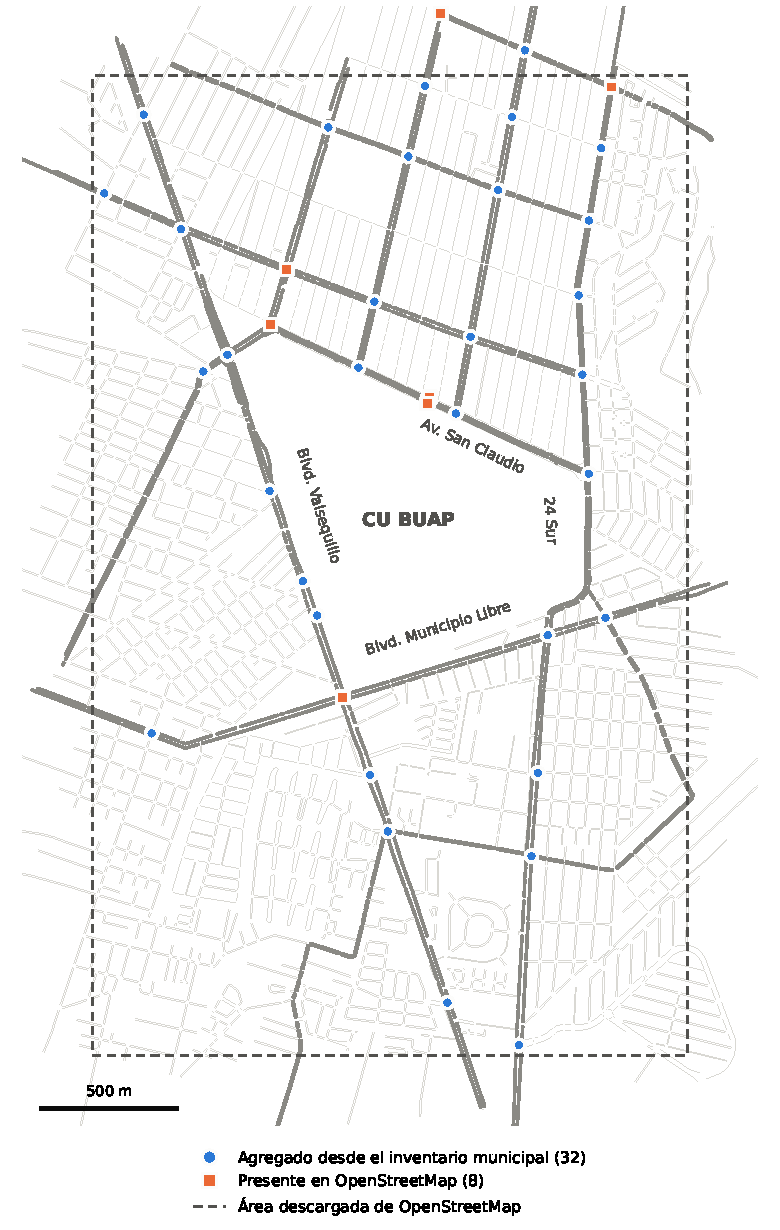
\includegraphics[width=0.62\linewidth]{AreaSemaforos.pdf}
\caption{Red vial simulada y sus 40 semáforos. Los círculos azules son
semáforos agregados desde el inventario municipal; los cuadros naranjas ya venían
en OpenStreetMap. La red se extiende fuera del área descargada porque conserva
completas las calles que cruzan el borde.}
\label{fig:area}
\end{figure}

\needspace{0.3\textheight}
\subsection{Datos}

\begin{table}[H]
\centering\small
\caption{Fuentes de datos del proyecto.}
\label{tab:datos}
\begin{tabularx}{\linewidth}{@{}l L l@{}}
\toprule
Fuente & Uso & Estado\\
\midrule
OpenStreetMap~\cite{osm} & Red vial: calles, carriles, sentidos, vueltas. Extracto congelado el 26/09/2026. & En uso\\
Inventario de Semáforos SEMOVINFRA 2021~\cite{inventario} & Ubicación de los semáforos reales. 3{,}283 postes en la ciudad, 156 en el área. & En uso\\
Inventario SEMOVINFRA, tabla 2020~\cite{inventario} & Comparación entre levantamientos (3{,}054 postes). & Guardado\\
Modelos de emisión y energía de SUMO~\cite{sumoemisiones,kurczveil} & Consumo y emisiones por vehículo. & Integrado en SUMO\\
Aforos vehiculares & Calibrar la demanda de hora pico. & Por conseguir\\
\bottomrule
\end{tabularx}
\end{table}

\subsection{Semáforos faltantes}

OpenStreetMap solo tenía 8 semáforos en la zona. El inventario municipal registra
36 intersecciones semaforizadas dentro del área. Como cada registro del
inventario es un poste y no una intersección, agrupamos los postes cercanos (a
35~m o menos, o a 80~m si nombran las mismas calles) y emparejamos cada grupo con el
cruce más cercano de la red, a menos de 30~m. Todas las intersecciones quedaron a
menos de 11~m de su cruce. Fuera del área, en los tramos que la red conserva, solo
agregamos semáforos en cruces completos: en la orilla la calle transversal suele
faltar, y un semáforo ahí solo agregaría demora artificial.

\begin{table}[!htbp]
\centering\small
\caption{Semáforos de la red simulada.}
\begin{tabular}{lr}
\toprule
& Cantidad\\
\midrule
Intersecciones del inventario dentro del área & 36\\
Intersecciones del inventario en la orilla, con cruce completo & 1\\
\midrule
Intersecciones del inventario en la red & 37\\
\quad ya presentes en OpenStreetMap & 5\\
\quad agregadas desde el inventario & 32\\
\quad con cabezas peatonales & 11\\
Semáforos de OpenStreetMap que no están en el inventario & 3\\
\midrule
\textbf{Semáforos en la red} & \textbf{40}\\
\bottomrule
\end{tabular}
\end{table}

Alrededor de CU hay 11 intersecciones semaforizadas: cinco sobre San Claudio (con
14 Sur, 18 Sur, la entrada a la Facultad de Derecho, 22 Sur y 24 Sur), dos sobre
Municipio Libre (con 24 Sur y con Valsequillo) y cuatro sobre Valsequillo (con
Universidad de Chapingo, UNAM, 63~F Oriente y 14 Sur). Son las candidatas a
operar con agentes; el resto de la red sigue con tiempo fijo. Dos pares están a
menos de 120~m entre sí y probablemente convenga controlar cada par como una sola
intersección; si el tiempo no alcanza, el plan es reducir el experimento a un arco
de 4 o 5 intersecciones sobre San Claudio.

En caso de cambiar de punto de interes, o querer probar otras zonas, se puede 
realizar el mismo procedimiento para cualquier otra zona de interés

\subsection{Reproducibilidad}

El proyecto vive en un repositorio con el extracto de OpenStreetMap congelado, el
inventario, las configuraciones y el código. Cualquier integrante reconstruye la
misma red con un solo comando; la construcción termina verificando que estén
todos los semáforos declarados y se detiene con error si falta alguno. Verificamos
que la red se reconstruye idéntica en un directorio limpio. La
figura~\ref{fig:sumo} muestra la red cargada en el simulador.

\begin{figure}[!htbp]
\centering
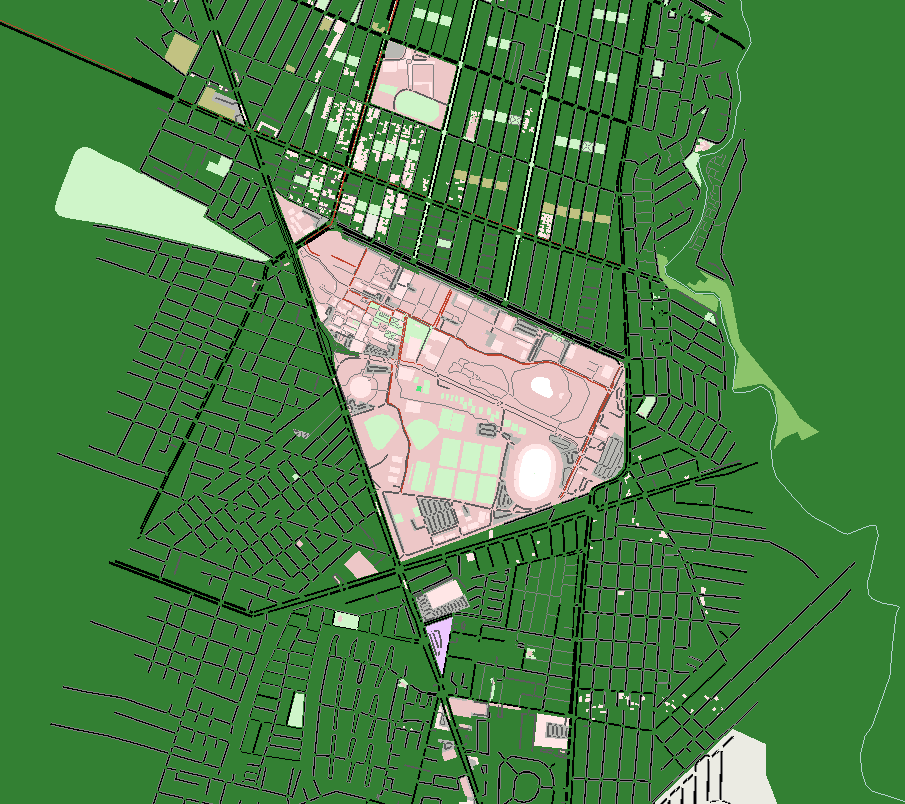
\includegraphics[width=0.7\linewidth]{VistaSumo.png}
\caption{La red alrededor de CU~BUAP en la interfaz gráfica de SUMO.}
\label{fig:sumo}
\end{figure}

% ------------------------------------------------------------------ 6
\section{Cómo lo vamos a evaluar}
\label{sec:eval}

\subsection{Controladores}

\begin{table}[!htbp]
\centering\small
\caption{Controladores comparados.}
\begin{tabularx}{\linewidth}{@{}c l L@{}}
\toprule
\# & Controlador & Papel\\
\midrule
1 & Tiempo fijo & Línea base obligatoria: cómo operan hoy los semáforos. Planes calculados con el método de Webster~\cite{webster}.\\
2 & DQN sin vecinos & Mismo agente, solo con observación local. Aísla cuánto aporta la coordinación.\\
3 & DQN con vecinos directos & Mensaje crudo de los vecinos inmediatos, sin fuerza de onda.\\
4 & DQN con onda causal difusa & El controlador principal: información de varios saltos ponderada por su fuerza de onda.\\
\bottomrule
\end{tabularx}
\end{table}

Los agentes DQN~\cite{dqn} se entrenan de forma independiente, uno por intersección
(\emph{Independent Q-Learning}~\cite{tan}), con Stable-Baselines3~\cite{sb3} sobre
un entorno Gymnasium construido a partir de sumo-rl~\cite{sumorl} y SUMO~\cite{sumo}.
\textbf{Las comparaciones 2 contra 3 y 3 contra 4 son los resultados más
importantes}: mismo agente y mismo código. La primera aísla cuánto aporta la
coordinación; la segunda, cuánto aporta la onda causal difusa sobre el mensaje
crudo.

\subsection{Métricas}

Todas se reportan contra tiempo fijo, como media y dispersión sobre al menos cinco
semillas de evaluación distintas de las de entrenamiento, con los mismos archivos
de demanda para todos los controladores.

\begin{table}[!htbp]
\centering\small
\caption{Métricas.}
\begin{tabularx}{\linewidth}{@{}l L@{}}
\toprule
Dimensión & Indicador\\
\midrule
Tráfico & Tiempo de espera medio, paradas por vehículo, longitud de cola.\\
Coordinación & Paradas en el corredor completo, tiempo de viaje de extremo a extremo.\\
Energía & kWh consumidos en el corredor, CO$_2$ evitado.\\
Peatones & Tiempo de espera peatonal, cruces con verde suficiente.\\
\bottomrule
\end{tabularx}
\end{table}

\subsection{Escenarios}

\begin{enumerate}
  \item Tráfico típico de hora pico.
  \item Tráfico asimétrico, con un sentido dominante: donde la coordinación debería rendir más.
  \item Pérdida del enlace con los vecinos: total (observaciones de vecinos en cero)
        y parcial (mensajes perdidos o retrasados en la onda).
\end{enumerate}

% ------------------------------------------------------------------ 7
\section{Qué esperamos obtener}

No tenemos resultados todavía. Estas son las hipótesis que el proyecto pone a
prueba; cualquiera puede resultar falsa, y en ese caso se reporta como tal.

\begin{enumerate}[label=\textbf{H\arabic*.}]
  \item El DQN sin vecinos reduce la espera media frente a tiempo fijo en hora pico.
  \item El DQN con vecinos reduce las paradas en el corredor y el tiempo de viaje de
        extremo a extremo frente al DQN sin vecinos, sobre todo con tráfico asimétrico.
  \item Al perder el enlace, el DQN con vecinos se degrada hacia el desempeño del DQN
        local, sin dejar de operar.
  \item La onda causal difusa reduce las paradas y el tiempo de viaje frente a los
        vecinos directos, sobre todo con pérdida parcial de mensajes,
        porque la fuerza de onda le indica al agente cuánto confiar en información
        lejana o vieja.
  \item Menos paradas y arranques se traducen en menos energía y emisiones por
        vehículo-kilómetro en el corredor.
\end{enumerate}

Entregables: la simulación reproducible, las comparaciones con sus figuras, el
estudio de ablación de la recompensa y los documentos del concurso (ficha técnica, memoria de cálculo y presentación).



% ------------------------------------------------------------------ referencias
\begin{thebibliography}{99}
\small
\setlength{\itemsep}{0pt}
\bibitem{sumo} P.~A. Lopez, M.~Behrisch, L.~Bieker-Walz, J.~Erdmann, Y.-P.~Flötteröd,
R.~Hilbrich, L.~Lücken, J.~Rummel, P.~Wagner y E.~Wießner. Microscopic traffic
simulation using SUMO. \emph{21st IEEE International Conference on Intelligent
Transportation Systems (ITSC)}, 2018, pp.~2575--2582.

\bibitem{colight} H.~Wei, N.~Xu, H.~Zhang, G.~Zheng, X.~Zang, C.~Chen, W.~Zhang,
Y.~Zhu, K.~Xu y Z.~Li. CoLight: Learning network-level cooperation for traffic
signal control. \emph{Proceedings of the 28th ACM International Conference on
Information and Knowledge Management (CIKM)}, 2019, pp.~1913--1922.

\bibitem{dqn} V.~Mnih et al. Human-level control through deep reinforcement
learning. \emph{Nature}, 518:529--533, 2015.

\bibitem{tan} M.~Tan. Multi-agent reinforcement learning: Independent vs.\
cooperative agents. \emph{Proceedings of the 10th International Conference on
Machine Learning (ICML)}, 1993, pp.~330--337.

\bibitem{sb3} A.~Raffin, A.~Hill, A.~Gleave, A.~Kanervisto, M.~Ernestus y
N.~Dormann. Stable-Baselines3: Reliable reinforcement learning implementations.
\emph{Journal of Machine Learning Research}, 22(268):1--8, 2021.

\bibitem{sumorl} L.~N. Alegre. SUMO-RL. Repositorio de software, 2019.
\url{https://github.com/LucasAlegre/sumo-rl}

\bibitem{webster} F.~V. Webster. \emph{Traffic Signal Settings}. Road Research
Technical Paper No.~39, HMSO, Londres, 1958.

\bibitem{kurczveil} T.~Kurczveil, P.~A. López y E.~Schnieder. Implementation of an
energy model and a charging infrastructure in SUMO. En \emph{Simulation of Urban
Mobility (SUMO 2013)}, LNCS 8594, Springer, 2014.

\bibitem{sumoemisiones} Eclipse SUMO. Documentación: modelos de emisiones.
\url{https://sumo.dlr.de/docs/Models/Emissions.html}

\bibitem{inventario} Gobierno Municipal de Puebla, Secretaría de Movilidad e
Infraestructura. \emph{Inventario de Semáforos SEMOVINFRA (histórico)}, versiones
2020 y 2021. Portal de Datos Abiertos de Puebla Capital, Licencia Libre Uso MX.
\url{https://datos.pueblacapital.gob.mx/dataset/inventario-de-sem\%C3\%A1foros}.
Consultado el 26/09/2026.

\bibitem{osm} Personas contribuyentes de OpenStreetMap. Datos bajo licencia ODbL.
\url{https://www.openstreetmap.org}. Extracto descargado el 26/09/2026.


\bibitem{evropeytsev2020} G.~Evropeytsev. \emph{Indirect Fuzzy-Causal Communication
Protocol for Vehicular Ad Hoc Networks}. Tesis doctoral, Instituto Nacional de
Astrofísica, Óptica y Electrónica (INAOE), Tonantzintla, Puebla, 2020.

\bibitem{evropeytsev2019} G.~Evropeytsev, S.~E. Pomares Hernández, J.~R. Pérez Cruz,
L.~M. Rodríguez Henríquez y E.~López Domínguez. A scalable indirect
position-based causal diffusion protocol for vehicular networks. \emph{IEEE
Access}, 7:14767--14778, 2019.

\bibitem{perez2014} J.~R. Pérez Cruz y S.~E. Pomares Hernández. Temporal alignment
model for data streams in wireless sensor networks based on causal dependencies.
\emph{International Journal of Distributed Sensor Networks}, 2014.

\bibitem{lamport} L.~Lamport. Time, clocks, and the ordering of events in a
distributed system. \emph{Communications of the ACM}, 21(7):558--565, 1978.

\bibitem{mamdani} E.~H. Mamdani y S.~Assilian. An experiment in linguistic synthesis
with a fuzzy logic controller. \emph{International Journal of Man-Machine
Studies}, 7(1):1--13, 1975.
\end{thebibliography}

\end{document}

%######################### FIN DE RESUMENPROYECTO.TEX ##########################
%###############################################################################
